\documentclass[11pt]{beamer}

% beamer posterの利用に関する設定
% A0 に合わせて 4 : 3 に
\usepackage[orientation=landscape,size=custom,width=84,height=119,scale=1.5]{beamerposter}

% メインフォントに関する設定
\usepackage{fontspec}
\setmainfont[Ligatures=TeX,BoldFont=Noto Serif Bold]{Noto Serif}
\setsansfont[Ligatures=TeX,BoldFont=Noto Sans Bold]{Noto Sans}
\usefonttheme[onlymath]{serif}

% CJKに対応させる
% 太字フォントを指定しないと疑似ボールドになる
\usepackage{xeCJK}
\setCJKmainfont[BoldFont=Noto Serif CJK JP Bold]{Noto Serif CJK JP}
\setCJKsansfont[BoldFont=Noto Sans CJK JP Bold]{Noto Sans CJK JP}

% 追加のフォント
\newfontfamily{\notosansmono}{Noto Sans Mono}

% その他
\usepackage{fancybox}
\usepackage{graphicx}
\usepackage{here}
\usepackage{mathtools}

% tikz
\usepackage{tikz}
\usepackage{pgfplots}
\usepackage{bchart}
\usetikzlibrary{positioning}
\usetikzlibrary{arrows.meta}

% beamerのテーマ・スタイルに関する設定
\setbeamertemplate{navigation symbols}{} % 右下のナビゲーションアイコンに消えてもらう
\setbeamercolor{normal text}{fg=black,bg=white}
\setbeamercolor{structure}{fg=red}

% blockのスタイル
\usepackage[most]{tcolorbox} % mostがないとenhanced(tikzを用いる装飾表現)が使えない
\setbeamertemplate{block begin}{
	\begin{tcolorbox}[ 
		enhanced,
		fonttitle=\bfseries,
		colframe=gray,
		colback=gray!5!,
		colbacktitle=gray!80,
		attach boxed title to top left={yshift=-2mm, xshift=2mm},
		title=\insertblocktitle
		]
		\vskip2mm
		}
		\setbeamertemplate{block end}{
	\end{tcolorbox}
	}

	\newenvironment{backblock}{%
		\begin{tcolorbox}[ 
			enhanced,
			fonttitle=\bfseries,
			colframe=gray,
			colback=gray!5!,
			colbacktitle=gray!80,
			attach boxed title to top left={yshift=-2mm, xshift=2mm}]
			\vskip2mm
			}{%
		\end{tcolorbox}
		}

		\newcommand{\titleblock}[3]{%
			\begin{center}
				\begin{tikzpicture}[
						font=\sffamily,
						scale=1.0,
						transform shape]
					\node[
						rectangle,
						text width=#1,
						text height=#2,
						fill=blue!20,
						draw=black,
						outer sep=1mm
					] at (0, 0) {};
					\node at (0, 0) {\textbf{#3}};
				\end{tikzpicture}
				\vspace*{-0.5em}
			\end{center}
			}

			% href
			\usepackage{hyperref}
			\hypersetup{
				colorlinks=true,
				linkcolor=blue,
				filecolor=magenta,
				urlcolor=cyan,
				pdfnewwindow=true}

			\newcommand{\forallngramx}{\forall n\mathchar`-\mathrm{gram}\ x}

			\begin{document}
			\begin{frame}[t]
				\vspace*{-1em}
				\begin{columns}[t]
					\begin{column}{0.14\linewidth}
						\begin{center}
							\fbox{\LARGE P4-25}
						\end{center}
					\end{column}
					\begin{column}{0.71\linewidth}
						\begin{center}
							%\begingroup \Large 文法誤り訂正の自動評価のための $n$-gram $F$-score \endgroup \vspace{0.5em} \\
							\begingroup \large 文法誤り訂正の自動評価のための原文・参照文・訂正文間の$n$-gram $F$-score \endgroup \vspace{0.5em} \\
							\textbf{\underline{古山翔太}} \begingroup \small(東工大/産総研,\ 岡崎研\ D2) \endgroup \hspace{0.5em}
							永田亮 \begingroup \small (甲南大/産総研) \endgroup \hspace{0.5em}
							高村大也 \begingroup \small(産総研)\endgroup	\hspace{0.5em}
							岡崎直観 \begingroup \small(東工大/産総研)\endgroup
						\end{center}
					\end{column}
					\begin{column}{0.14\linewidth}
					\end{column}
				\end{columns}
				\vspace*{1em}

				\begin{columns}[t]
					\begin{column}{0.50\linewidth}
						\titleblock{180}{50}{概要}
						\begin{backblock}
							\begin{itemize}
								\item 文法誤り訂正とは? 文書中の誤りを訂正するタスク。
									\begin{itemize}
										\item 例: ``\textit{What is you?}'' $\to$ ``\textit{Who are you?}''
									\end{itemize}
								\item システムの出力への良い自動評価手法がほしい。
									\begin{itemize}
										\item システムの質を人手で評価するのは避けたい。
									\end{itemize}
								\item M${}^2$とその派生が広く使われている。
									\begin{itemize}
										\item 文間のフレーズアライメントを取り、訂正の個数を数え、$F$-scoreを計算。
									\end{itemize}
								\item M${}^2$系の問題点は?
									\begin{itemize}
										\item アライメントの計算に時間がかかる。また、アノテーションされたデータや、その他のツールが必要となる。
									\end{itemize}
								\item 提案手法 GREEN
									\begin{itemize}
										\item 文を$n$-gramの多重集合とみなし、文間の編集を集合操作で抽出する。
											\begin{itemize}
												\item アライメントの計算が不要。
											\end{itemize}
										\item 原文から参照文の編集、原文から訂正文の編集を比較し、$F$-scoreを計算。 
										\item 既存の手法より人手評価と高い相関を示した。
									\end{itemize}
							\end{itemize}
						\end{backblock}

						\titleblock{180}{50}{手法}
						\begin{backblock}
							\begin{itemize}
								\item 提案手法GREENは、文を最大長$N$までの$n$-gramの多重集合として扱う。
									%\begin{itemize}
									%\item
									(例: 文$A=$``\textit{a a b}''は、$N=2$で、$\{\textit{a}, \textit{a}, \textit{b}, \textit{a a}, \textit{a b}\}$。)
									%\end{itemize}
								\item 原文$S$, 参照文$R$, 訂正文$C$を多重集合で表し、ベン図を用いて文中の$n$-gramに対して7分類を行う。
							\end{itemize}
							\begin{figure}[t]
								\centering
								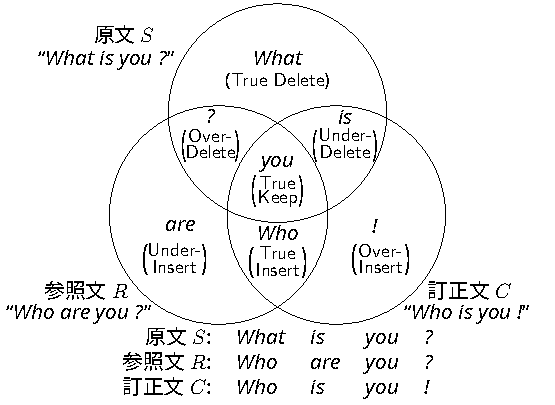
\includegraphics[width=30cm]{venn-1.pdf}
							\end{figure}
							\begin{table}[t]
								\centering
								\begin{tabular}{l|l|ll}
									\hline
									領域 & 名前 & $S \to R$ & $S \to C$ \\
									\hline
									$S \cap \overline{R} \cap \overline{C} $ &
									\makebox[6.3em][l]{\textsf{True Delete}}~(\textsf{TD}) &
									Delete & Delete \\
									$\overline{S} \cap R \cap C$ &
									\makebox[6.3em][l]{\textsf{True Insert}}~(\textsf{TI}) &
									Insert & Insert \\
									$S \cap R \cap C$ &
									\makebox[6.3em][l]{\textsf{True Keep}}~(\textsf{TK}) &
									Keep & Keep \\
									\hline
									$S \cap R \cap \overline{C}$ &
									\makebox[6.3em][l]{\textsf{Over-Delete}}~(\textsf{OD}) &
									Keep & Delete \\
									$\overline{S} \cap \overline{R} \cap C$ &
									\makebox[6.3em][l]{\textsf{Over-Insert}}~(\textsf{OI})
									& なし & Insert \\
									\hline
									$S \cap \overline{R} \cap C$ &
									\makebox[6.3em][l]{\textsf{Under-Delete}}~(\textsf{UD}) &
									Delete & Keep \\
									$\overline{S} \cap R \cap \overline{C}$ & \makebox[6.3em][l]{\textsf{Under-Insert}}~(\textsf{UI}) &
									Insert & なし \\
									\hline
								\end{tabular}
							\end{table}
							\begin{itemize}
								\item 多重集合の重複度(頻度)$m_A(x)$を用いる。(例: $m_A(\textit{a})=2$)
								\item 多重集合上の演算(積$\cap$、和$\cup$、差$\setminus$)を定義。
							\end{itemize}
							\begin{align*}
								m_{A \cap B} (x) & = \min (m_A (x), m_B (x)) \\
								m_{A \cup B} (x) & = \max (m_A (x), m_B (x)) \\
								m_{A \setminus B} (x) & = \max (m_A (x) - m_B (x), 0)
							\end{align*}
							\vspace*{-1em}
							\begin{itemize}
								\item 原文$S$、参照文$R$、訂正文$C$の各$n$-gram $x$を、ベン図を用いた7分類で数え上げる。
							\end{itemize}
							\begin{align*}
								\textsf{TD}_{S, R, C} (x)
								= & m_{S \cap \overline{R} \cap \overline{C}} (x)
								= m_{S \setminus (R \cup C)} (x) \\
								= & \max\{m_S (x) - \max(m_R (x), m_C (x)), 0\} \\[4\jot]
								\textsf{TI}_{S, R, C} (x)
								= & m_{\overline{S} \cap R \cap C} (x)
								= m_{(R \cap C) \setminus S} (x) \\
								= & \max\{\min(m_R (x), m_C (x)) - m_S (x), 0\} \\[4\jot]
								\textsf{TK}_{S, R, C} (x)
								= & m_{S \cap R \cap C}(x)
								= \min(m_S(x), m_R(x), m_C (x)) \\[4\jot]
								\textsf{OD}_{S, R, C} (x)
								= & m_{S \cap R \cap \overline{C}} (x)
								= m_{(S \cap R) \setminus C} (x) \\
								= & \max\{\min(m_S (x), m_R (x)) - m_C (x), 0\} \\[4\jot]
								\textsf{OI}_{S, R, C} (x)
								= & m_{\overline{S} \cap \overline{R} \cap C} (x)
								= m_{C \setminus (S \cup R)} (x) \\
								= & \max\{m_C (x) - \max(m_S (x), m_R (x)), 0\} \\[4\jot]
								\textsf{UD}_{S, R, C} (x)
								= & m_{S \cap \overline{R} \cap C} (x)
								= m_{(S \cap C) \setminus R} (x) \\
								= & \max\{\min(m_S (x), m_C (x)) - m_R (x), 0\} \\[4\jot]
								\textsf{UI}_{S, R, C} (x)
								= & m_{\overline{S} \cap R \cap \overline{C}} (x)
								= m_{R \setminus (S \cup C)} (x) \\
								= & \max\{m_R (x) - \max(m_S (x), m_C (x)), 0\}
							\end{align*}
						\end{backblock}
					\end{column}

					\begin{column}{.50\linewidth}
						\vspace*{-1.5em}
						\begin{backblock}
							\begin{itemize}
								\item 各$n$で$S, R, C$ごとの\textsf{True Positive}~(\textsf{TP}), \textsf{False Positive}~(\textsf{FP}), \textsf{False Negative}~(\textsf{FN})を計算する。
							\end{itemize}
							\begin{align*}
								\textsf{TP}_{n, S, R, C} = & \sum_{\mathclap{\forallngramx}} \left( \textsf{TD}_{S,R,C} (x) + \textsf{TI}_{S,R,C} (x) + \textsf{TK}_{S,R,C} (x) \right) \\
								\textsf{FP}_{n, S, R, C} = & \sum_{\mathclap{\forallngramx}} \left( \textsf{OD}_{S,R,C} (x) + \textsf{OI}_{S,R,C} (x) \right) \\
								\textsf{FN}_{n, S, R, C} = & \sum_{\mathclap{\forallngramx}} \left( \textsf{UD}_{S,R,C} (x) + \textsf{UI}_{S,R,C} (x) \right)
							\end{align*}
							\vspace*{-0.5em}
							\begin{itemize}
								\item 各$n$でコーパス全体($\mathbb{S} = (S_1, \ldots), \mathbb{R} = (R_1, \ldots), \mathbb{C} = (C_1, \ldots)$)でのprecision, recallの幾何平均を取り、GREENの$F_{\beta}$値を求める。
							\end{itemize}
							\begin{align*}
								\mathrm{precision} (N, \mathbb{S}, \mathbb{R}, \mathbb{C}) = & \left( \prod_{n=1}^{N}
								\frac{
									\sum_{i} \textsf{TP}_{n, S_i, R_i, C_i}
								}{
									\sum_{i} \left( \textsf{TP}_{n, S_i, R_i, C_i} + \textsf{FP}_{n, S_i, R_i, C_i} \right)
								}
								\right)^{\tfrac{1}{N}} \\
								\mathrm{recall} (N, \mathbb{S}, \mathbb{R}, \mathbb{C}) = & \left( \prod_{n=1}^{N}
								\frac{
									\sum_{i} \textsf{TP}_{n, S_i, R_i, C_i}
								}{
									\sum_{i} \left( \textsf{TP}_{n, S_i, R_i, C_i} + \textsf{FN}_{n, S_i, R_i, C_i} \right)
								}
								\right)^{\tfrac{1}{N}}
							\end{align*}
							\begin{align*}
								\mathrm{GREEN}_{\beta} (N, \mathbb{S}, \mathbb{R}, \mathbb{C}) = &
								\frac{
									(1+\beta^2) \mathrm{precision} (N, \mathbb{S}, \mathbb{R}, \mathbb{C})  \mathrm{recall} (N, \mathbb{S}, \mathbb{R}, \mathbb{C})
								}{
									\beta^2 \mathrm{precision} (N, \mathbb{S}, \mathbb{R}, \mathbb{C}) + \mathrm{recall} (N, \mathbb{S}, \mathbb{R}, \mathbb{C})
								}
							\end{align*}
							\begin{itemize}
								\item 複数の参照文($R_{i_1},\ldots,R_{i_m}$)がある場合は、文単位でスコアを最大にする$\hat{R}_i$を選ぶ。
							\end{itemize}
							\begin{equation*}
								\hat{R}_i = \operatorname*{argmax}_{\mathclap{R \in \{R_{i_1}, \ldots, R_{i_m}\}}} \mathrm{GREEN}_{\beta}(N, (S_i), (R), (C_i))
							\end{equation*}
						\end{backblock}

						\titleblock{180}{50}{実験}
						\begin{backblock}
							\begin{itemize}
								\item CoNLL-2014評価タスクでの評価
									\begin{itemize}
										\item Corpus-level評価を行い、Expected Wins法の\alert{人手評価値との相関係数}、1システムに対する\alert{1回の評価の実行時間}の平均を計測した。
										\item アライメントによる$F$-scoreは、precision-orientedな評価を行うため、$\beta = 0.5$を用いる。$n$-gramによる手法は、参照データ数のバイアスを緩和するため、recall-orientedな評価を行い、$\beta = 2.0$を用いる。
										\item $n$-gramの計測の分割は、単語単位、文字単位で行い、それぞれ、\\word+手法名、char+手法名と表記する。
										\item charGREENは、既存手法より高い相関を示す。
										\item GREENは、既存手法よりも高速に評価を行える。
										\item M${}^2$は人手でアノテーションしたアライメントを必要とする。ERRANT、CLEMEは品詞タグ付けによるアライメントを行う。PT-M${}^2$はBERTを用いる。GREENは追加のデータやツールが不要かつ高速で、高性能である。
									\end{itemize}
							\end{itemize}
							\begin{table}[!t]
								\centering
								\begin{tabular}{lrrr}
									\hline
									& \multicolumn{1}{c}{$r$} & \multicolumn{1}{c}{$\rho$} & \multicolumn{1}{c}{時間~(秒)} \\ \hline
									\multicolumn{4}{l}{アライメントによる$F$-score} \\
									M${}^2$ & 0.623 & 0.687 & 4.34 \\
									ERRANT & 0.644 & 0.687 & 12.35 \\
									PT-M${}^2$ & 0.686 & 0.786 & 109.82 \\
									CLEME & 0.648 & 0.709 & 10.15 \\
									\hline
									\multicolumn{4}{l}{$n$-gramによるprecision} \\
									wordGLEU & 0.696 & 0.445 & 2.69 \\
									charGLEU & 0.606 & 0.593 & 5.00 \\
									\hline
									\multicolumn{4}{l}{$n$-gramによる$F$-score} \\
									wordGREEN & 0.741 & 0.698 & \textbf{0.55} \\
									charGREEN & \textbf{0.786} & \textbf{0.813} & 1.94 \\ \hline
								\end{tabular}
							\end{table}
						\end{backblock}

						\begin{backblock}
							\begin{itemize}
								\item 評価手法ごとの違いは?
									\begin{itemize}
										\item \makebox[3.5em][l]{\textsf{AMU}}: CoNLL-2014タスクで最も人手評価値が高い出力
										\item \makebox[3.5em][l]{\textsf{INPUT}}: CoNLL-2014タスクの入力文をそのまま出力とする
										\item \makebox[3.5em][l]{\textsf{IPN}}: CoNLL-2014タスクで最も人手評価値が低い出力
										\item \makebox[3.5em][l]{\textsf{NULL}}: すべての入力に対して、空の文を出力とする
									\end{itemize}
								\item アライメントによる$F$-scoreは、悪い出力を高く評価してしまうことがある。
							\end{itemize}
							\begin{table}[t]
								\centering
								\begin{tabular}{lrrrr}
									\hline
									& \multicolumn{1}{c}{AMU} & \multicolumn{1}{c}{INPUT} & \multicolumn{1}{c}{IPN} & \multicolumn{1}{c}{NULL} \\
									\hline
									\multicolumn{5}{l}{アライメントによる$F$-score} \\
									M${}^2$ & 35.01 & 0.00 & 7.09 & 28.01 \\
									ERRANT & 31.97 & 0.00 & 5.95 & 0.20 \\
									PT-M${}^2$ & 35.94 & 0.00 & 5.72 & 2.44 \\
									CLEME & 25.14 & 0.00 & 4.41 & 33.44 \\
									\hline
									\multicolumn{5}{l}{$n$-gramによるprecision} \\
									wordGLEU & 58.08 & 56.34 & 55.08 & 0.00 \\
									\hline
									\multicolumn{5}{l}{$n$-gramによる$F$-score} \\
									wordGREEN & 79.26 & 76.93 & 76.31 & 43.46 \\
									\hline
									人手評価 & 62.84 & 45.64 & 29.99 & \multicolumn{1}{c}{-} \\
									\hline
								\end{tabular}
							\end{table}
						\end{backblock}
					\end{column}
				\end{columns}
			\end{frame}
		\end{document}
